\section{Multi-Robot Approach for Weld Cost Minimization}

In the approach section(cite section) we discussed how introduction of another robot can increase the number of degrees of freedom and hence allow the robot to perform more complex manipulations. Increasing the degree of complexity of motion can allow us to implement better optimization as well as solve the problems of unreachability and singularity. In this chapter we will discuss the integration of a 2 degrees of freedom rotary table into the existing architecture and how that is utilized to optimize the welding task. 

\subsection{Modeling the Rotary Table}
The existing implementation only contained kinematic description of the 6 axis manipulator with the weld tool tip. In the following subsections, we present a model of the 2 degree of freedom rotary table, along with the kinematic description and present the improved architectural model.
\subsubsection{Architecture of RobotKit}
The following architectural diagram(\ref{fig:img9}) has been color coded for better understanding. Blue represents the core functionalities of RobotKit. Red represents the kinematics and visualization models on which the improvements are implemented. Green represents external configuration files that are loaded inside RobotKit. Yellow represents the OMPL based planning library and pink represents the user interface block. \\
In the existing architecture the Kernel block creates instances of the kinematics and visualization models of the 6 Dof robot, which update the simulation environment based on the data input from the Information Exchange Pipeline. The planner interface class takes input from the kernel and the information exchange pipeline and user input for welding task. It then creates a planning problem and sends it to the OMPL based planning library. The communication between the planner interface and the planning library takes place using dll files. The project configuration file loads information about the dH parameters of the robot, position of the work piece and other relevant objects and in the weld cell. 

\begin{figure}[!htbp] %  figure placement: here, top, bottom, or page
 \centering
   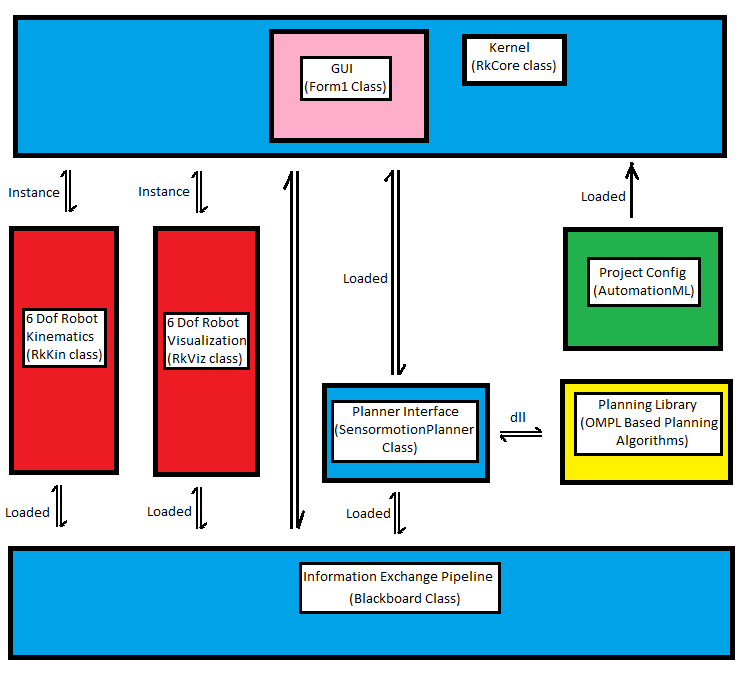
\includegraphics[width=9cm]{images/Original_arch.png}
   \caption[Exisitng Architecture of RobotKit(cite rk)]
   {Exisitng Architecture of RobotKit}  
\label{fig:img9}
\end{figure}

In the following architecture diagram (\ref{fig:img10}) the exact blocks which have been updated are highlighted. The kinematic and the visualization models now also includes definition of rotary table. The project configuration file (highlighted in green) has also been updated to include the dH parameters of the rotary table. 
\begin{figure}[!htbp] %  figure placement: here, top, bottom, or page
 \centering
   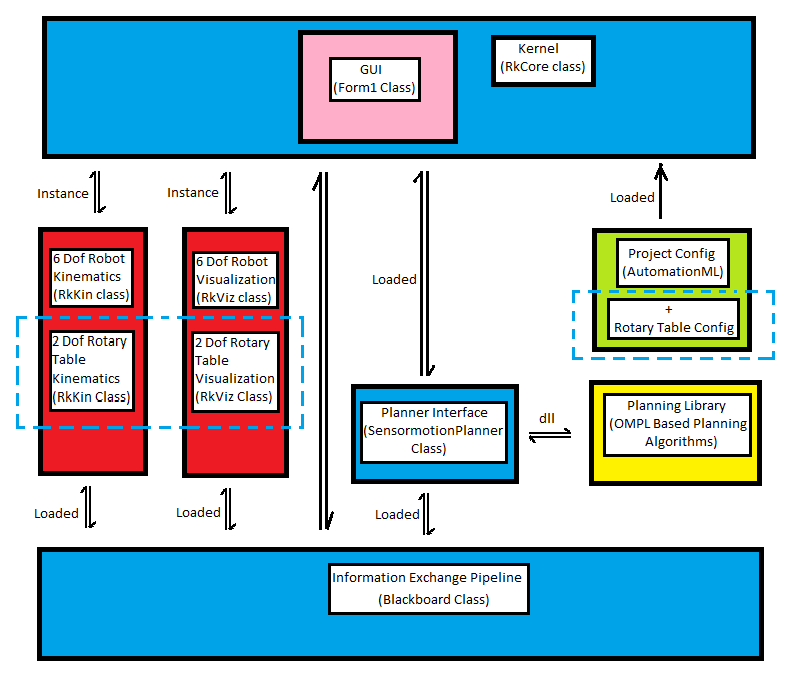
\includegraphics[width=9cm]{images/new_arch.png}
   \caption[Updated Architecture of RobotKit(cite rk)]
   {Updated Architecture of RobotKit}  
\label{fig:img10}
\end{figure}
 

\subsubsection{Generating 3D Models for Simulation}
In order to update the simulation environment, 3D CAD models of the rotary table were created using Solidworks software(cite solidworks), based on the data-sheet specifications. In order to make the simulation mimic the real functioning of the rotary table, the table was divided into 3 separate CAD objects; base, middle joint and top plate. The images for the same are presented herewith. 

\begin{figure}[!htbp] %  figure placement: here, top, bottom, or page
\begin{subfigure}{\linewidth}
   \frame{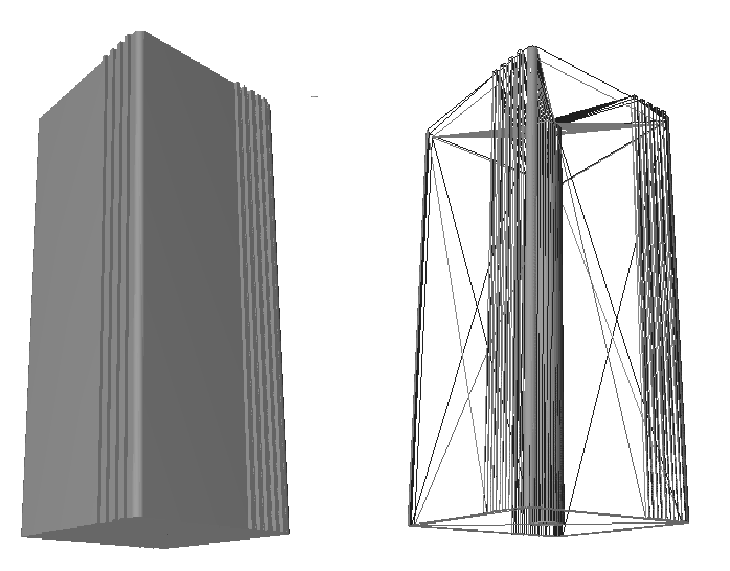
\includegraphics[width=.5\linewidth]{images/Base.png}}
   \frame{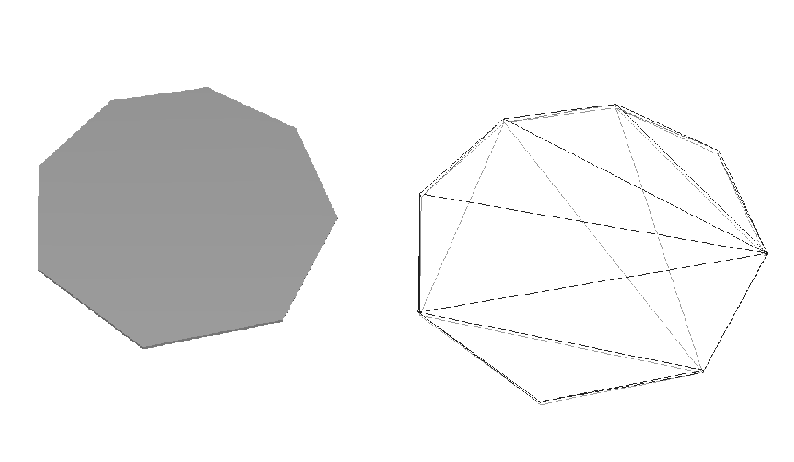
\includegraphics[width=.5\linewidth]{images/Top.png}}
      \caption[dd]{Base and Top Joint models}
   \end{subfigure}\par\medskip
   \begin{subfigure}{\linewidth}
   \centering
   \frame{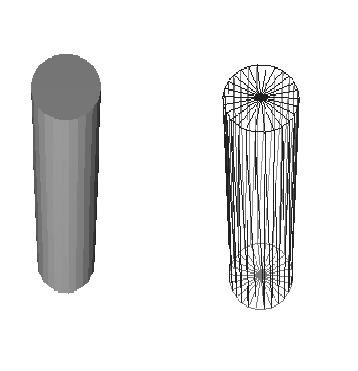
\includegraphics[width=.5\linewidth]{images/Mid.png}}
   \caption[dd]{Middle Joint model}
   \end{subfigure}
\caption[dd]{CAD models of the Rotary Table: Base, Middle and Top}
\label{fig:img11}
\end{figure}
 

\subsubsection{Kinematic Description of the Rotary Table}

The kinematic description of the 2 Dof Rotary table was created using the standard DH parameter approach. The DH parameters as specified in the Reis welding cell data-sheet(cite datasheet) are presented in the following table \ref{tab2}
\begin{table}[!htbp]
\centering
\scalebox{1.2}{%
\frame{\begin{tabular}{@{}lllll@{}}
\toprule
i & $\alpha_{i-1}$ & a\_\{i-1\} & d\_\{i\} & $\theta_{i}$ \\ \midrule
1 & 0              & 0          & 0        & $\theta_{1}$ \\
2 & -90            & 0          & 150 mm     & $\theta_{2}$
\end{tabular}%
}}
\caption{DH parameter of Rotary Table}
\label{tab2}
\end{table}
\\
The next step is to construct the link frames of the joints of the table in accordance with the approach mentioned in (cite Introduction to robotics, jacob book). The frames were plotted in Cartesian space with actual values from the real robot system. The values are the actual coordinates of the joint with respect to the global coordinate frame. Since the rotary table present in the welding cell has 2 Dof, we take Joint 0 as a reference frame, which coincides with the frame of Joint 1. According to the Reis welding cell data-sheet(use cite doc), the axis of rotation of Joint 1 of the rotary table is same as the X axis of the robot frame of the 6 dof manipulator and the axis of rotation of Joint 2 is same as the Z axis of the robot frame of the 6 dof manipulator. \\
In the following figure \ref{fig:img12} the world and robot frames along with the joint frames of the rotary table in the Cartesian coordinate frame are plotted. 
\begin{figure}[!htbp] %  figure placement: here, top, bottom, or page
 \centering
   \frame{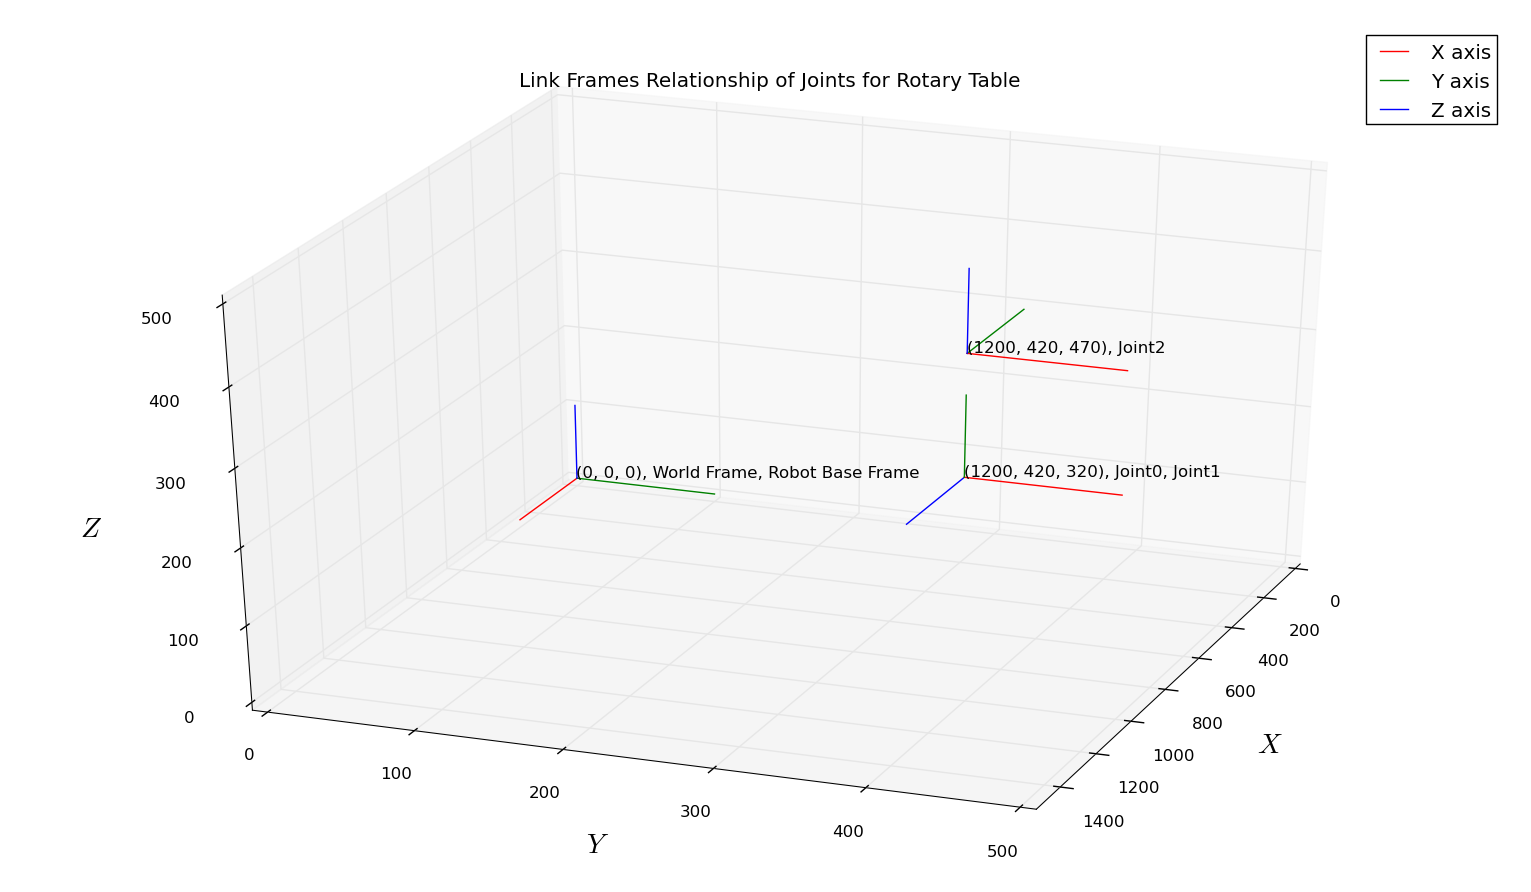
\includegraphics[width=12cm]{images/Frames_jnttab.png}}
   \caption{Link Frame Relationship of Joints of Rotary Table}  
\label{fig:img12}
\end{figure}

Based on the DH parameters from table \ref{tab2} we now construct the forward kinematic chain. 
\begin{equation}
\label{eq20}
_{0}^{1}\textrm{T} = \begin{bmatrix} \cos\theta_{i} & -\sin \theta_{i} & 0 & 0\\ \sin \theta_{i} & \cos \theta_{i} & 0 & 0\\ 0 & 0 & 1 & 0\\ 0 & 0 & 0 & 1 \end{bmatrix}
\end{equation}

\begin{equation}
\label{eq21}
_{2}^{1}\textrm{T} = \begin{bmatrix} \cos\theta_{i} & -\sin \theta_{i} & 0 & 0\\ 0 & 0 & 1 & 150\\ -\sin \theta_{i} & -\cos\theta_{i} & 0 & 0\\ 0 & 0 & 0 & 1 \end{bmatrix}
\end{equation}

\begin{equation}
\label{eq22}
\textrm{T}_{table} =_{2}^{0}\textrm{T}_{1}^{0}\textrm{T}._{2}^{1}\textrm{T} = \begin{bmatrix} \cos^{2}\theta_{i}& -\cos\theta_{i}.\sin\theta_{i} & -\sin\theta_{i} & -150*\sin\theta_{i}\\ \cos\theta_{i}.\sin\theta_{i} & -\sin^{2}\theta_{i} & \cos\theta_{i} & 150*\cos\theta_{i}\\ -\sin\theta_{i} & -\cos\theta_{i}& 0 & 0\\ 0& 0& 0& 1\end{bmatrix}
\end{equation}

\subsubsection{Workpiece Transformation}

Since the main objective of moving the rotary table is to move the work piece, a transformation function is also necessary to simulate the changed position of the work piece in accordance with the motion of the table. 

\begin{algorithm}[!htbp]
	\caption{Transformation of Work Piece position wrt Table Position}
	\label{algo2}
	\textbf{Given:} $ \text{Original }(\textit{$_{T}^{W}P$}, \textit{$_{T}^{W}O$})\text{pose and orientation information}  \bigwedge \text{ new}\\(\textit{$_{T}^{W}P_{new}$}, \textit{$_{T}^{W}O_{new}$}) \text{pose and orientation information} \text{ of table wrt. to world frame }\\ \text{ and current position and orientation } (\textit{$_{WP}^{W}P$}, \textit{$_{WP}^{W}O$}) \text{information of work piece wrt.} \\ \text{world frame} $ \\ \\
	\textbf{Output:} $\text{New}(\textit{$_{WP}^{W}P_{new}$},\textit{$_{WP}^{W}O_{new}$}) \text{position and orientation  information} \\ \text{of work piece wrt. world frame}$\\
	
	\begin{algorithmic}[1]
		\State $\textit{$_{T}^{W}T$} \gets Converttomatrix(\textit{$_{T}^{W}P$},\textit{$_{T}^{W}O$})$
		\State $\textit{$_{WP}^{W}P$} \gets Converttomatrix(\textit{$_{WP}^{W}P$},\textit{$_{WP}^{W}O$})$
		\State $\textit{$_{T}^{W}T_{new}$} \gets Converttomatrix(\textit{$_{T}^{W}P_{new}$}, \textit{$_{T}^{W}O_{new}$})$ \\
		\If{[${Initializing program}$]}
		\State $\textit{$_{WP}^{T}T_{ref}$} \gets \textit{$_{T}^{W}T^{-1}$} * \textit{$_{WP}^{W}T$}$
		\EndIf \\
		\If{[$\text{user offset work piece position}$]}
		\State $\textit{$_{WP}^{T}T^{'}$} \gets \textit{$_{T}^{W}T^{-1}$} * \textit{$_{WP}^{W}T^{'}$}$
		\State $\textit{$_{WP}^{T}T_{ref}$} \gets $\textit{$_{WP}^{T}T^{'}$}
		\EndIf \\
		
		\State $\textit{$_{WP}^{W}T_{new}$} \gets \textit{$_{T}^{W}T_{new}^{-1}$} * \textit{$_{WP}^{T}T_{ref}$}$\\
		\State $\textit{$_{WP}^{W}P_{new}$} \gets position(\textit{$_{WP}^{W}T_{new}$})$
		\State $\textit{$_{WP}^{W}O_{new}$} \gets matrixtoeulerangles(\textit{$_{WP}^{W}T_{new}$})$\\
		\If{[$Edge to be welded selected$]}
		\State $SelectedEdgeTransform()$
		\EndIf \\
		\textbf{return:} $\textit{$_{WP}^{W}P_{new}$},\textit{$_{WP}^{W}O_{new}$}$
	\end{algorithmic}
\end{algorithm}
\newpage
\subsubsection{Selected Edge Transformation}

\begin{algorithm}
	\caption{Transformation of Selected Edge wrt Work Piece Position}
	\label{algo2}
	\textbf{Given:} $ \text{Original pose and orientation information of start(\textit{$_{SP}^{W}P$}, \textit{$_{SP}^{W}O$}) and goal} \\ \text{points(\textit{$_{GP}^{W}P$}, \textit{$_{GP}^{W}O$}) }  \bigwedge \text{ new}(\textit{$_{WP}^{W}P_{new}$}, \textit{$_{WP}^{W}O_{new}$}) \text{pose and orientation information} \\ \text{ of work piece wrt. to world frame } \text{ and old position and orientation }\\ (\textit{$_{WP}^{W}P$}, \textit{$_{WP}^{W}O$}) \text{information of work piece wrt. world frame} $ \\ 
	\textbf{Output:} $\text{New pose and orientation information of start(\textit{$_{SP}^{W}P_{new}$}, \textit{$_{SP}^{W}O_{new}$}) and } \\ \text{goal points(\textit{$_{GP}^{W}P_{new}$}, \textit{$_{GP}^{W}O_{new}$}) }$\\
	
	\begin{algorithmic}[1]
		\State $\textit{$_{SP}^{W}T$} \gets Converttomatrix(\textit{$_{SP}^{W}P$},\textit{$_{SP}^{W}O$})$
		\State $\textit{$_{GP}^{W}T$} \gets Converttomatrix(\textit{$_{GP}^{W}P$},\textit{$_{GP}^{W}O$})$
		\State $\textit{$_{WP}^{W}T$} \gets Converttomatrix(\textit{$_{WP}^{W}P$},\textit{$_{WP}^{W}O$})$
		\State $\textit{$_{WP}^{W}T_{new}$} \gets Converttomatrix(\textit{$_{WP}^{W}P_{new}$}, \textit{$_{WP}^{W}O_{new}$})$ 
		\For{[$each selected edge$]} 
		\If{[${Initializing program}$]}
		\State $\textit{$_{SP}^{WP}T_{ref}$} \gets \textit{$_{WP}^{W}T^{-1}$} * \textit{$_{SP}^{W}T$}$
		\State $\textit{$_{GP}^{WP}T_{ref}$} \gets \textit{$_{WP}^{W}T^{-1}$} * \textit{$_{GP}^{W}T$}$
		\EndIf 
		\If{[$\text{user offset work piece position}$]}
		\State $\textit{$_{SP}^{WP}T^{'}$} \gets \textit{$_{WP}^{W}T_{new}^{-1}$} * \textit{$_{SP}^{W}T$}$
		\State $\textit{$_{GP}^{WP}T^{'}$} \gets \textit{$_{WP}^{W}T_{new}^{-1}$} * \textit{$_{GP}^{W}T$}$
		\State $\textit{$_{SP}^{WP}T_{ref}$} \gets $\textit{$_{SP}^{WP}T^{'}$}
		\State $\textit{$_{GP}^{WP}T_{ref}$} \gets $\textit{$_{SP}^{WP}T^{'}$}
		\EndIf 		
		\State $\textit{$_{SP}^{W}T_{new}$} \gets \textit{$_{WP}^{W}T_{new}^{-1}$} * \textit{$_{SP}^{WP}T_{ref}$}$
		\State $\textit{$_{GP}^{W}T_{new}$} \gets \textit{$_{WP}^{W}T_{new}^{-1}$} * \textit{$_{GP}^{WP}T_{ref}$}$
		
		\State $\textit{$_{SP}^{W}P_{new}$} \gets position(\textit{$_{SP}^{W}T_{new}$})$
		\State $\textit{$_{SP}^{W}O_{new}$} \gets matrixtoeulerangles(\textit{$_{SP}^{W}T_{new}$})$
		\State $\textit{$_{GP}^{W}P_{new}$} \gets position(\textit{$_{GP}^{W}T_{new}$})$
		\State $\textit{$_{GP}^{W}O_{new}$} \gets matrixtoeulerangles(\textit{$_{GP}^{W}T_{new}$})$\\
		
		\EndFor \\
		\textbf{return:} $\textit{$_{SP}^{W}P_{new}$},\textit{$_{SP}^{W}O_{new}$},\textit{$_{GP}^{W}P_{new}$},\textit{$_{GP}^{W}O_{new}$}$
	\end{algorithmic}
\end{algorithm}
\newpage
\subsection{Cost Function Formulation}
Two different cost functions were formulated and finally a weighted combination of the two was created, to form the final cost function. The plots of the cost functions were created by running the planner for every different orientations of the table
\subsubsection{Cost Function based on Tooltip orientation relative to Workpiece edge}
In (cite PPR paper) the authors define the optimal TCP orientation; 45$\deg$ with respect to the work piece edge for generating a weld path. For our initial cost estimate we consider the difference between the actual TCP orientation and the defined optimal TCP orientation. The greater the difference, higher the cost and vice-versa. The difference in orientation is calculated based on the difference of the quaternion values of the two orientations.\\
Based on the definition of optimal cost, we plot the cost function for 2 different work pieces and two different welding edges. Based on the orientation of the welding edge, the joint angles of the table for which the cost is minimal is also varied. The cost values are fixed between a of range of 0 to 100, so that we can carry out a comparative evaluation, among the different use cases.
\paragraph{1st Work Piece}
\subparagraph{1st Edge}

\begin{figure}[!htbp] %  figure placement: here, top, bottom, or page
 \centering
   \frame{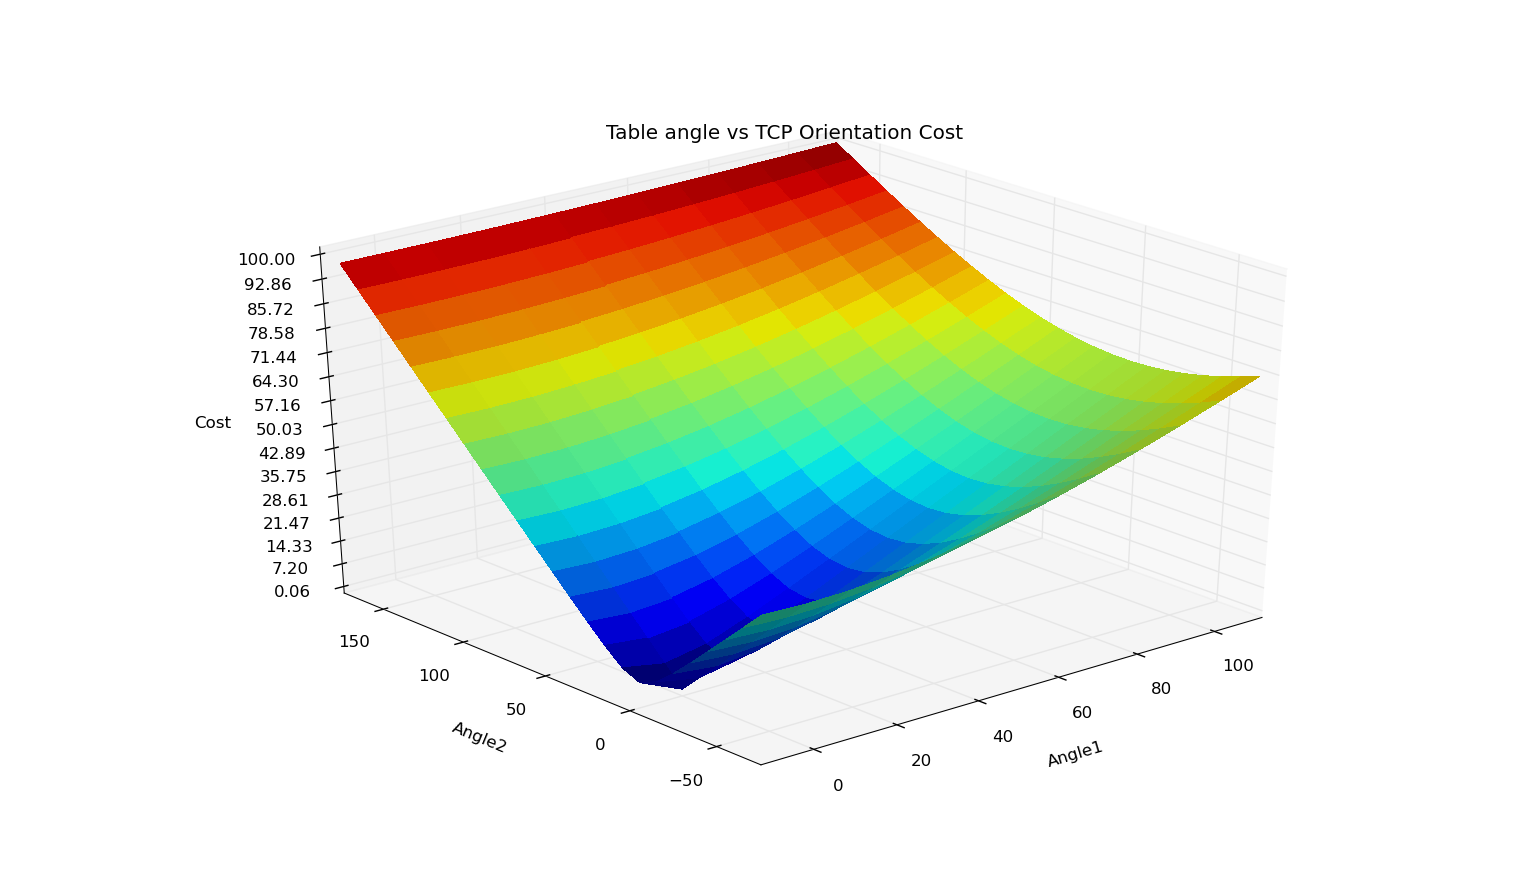
\includegraphics[width=\textwidth]{images/cost_plot1.png}}
   \caption{Cost Plot of Table Angle vs TCP Orientation}  
\label{fig:img13}
\end{figure}
The edge to be welded is marked in yellow(cite fig). In this cost plot(ref img), the minimum cost is obtained when the joints of the table are both at 0$\deg$. In the plot, red represents a higher cost region while blue represents lower cost.
\subparagraph{2nd Edge}
\begin{figure}[!htbp] %  figure placement: here, top, bottom, or page
 \centering
   \frame{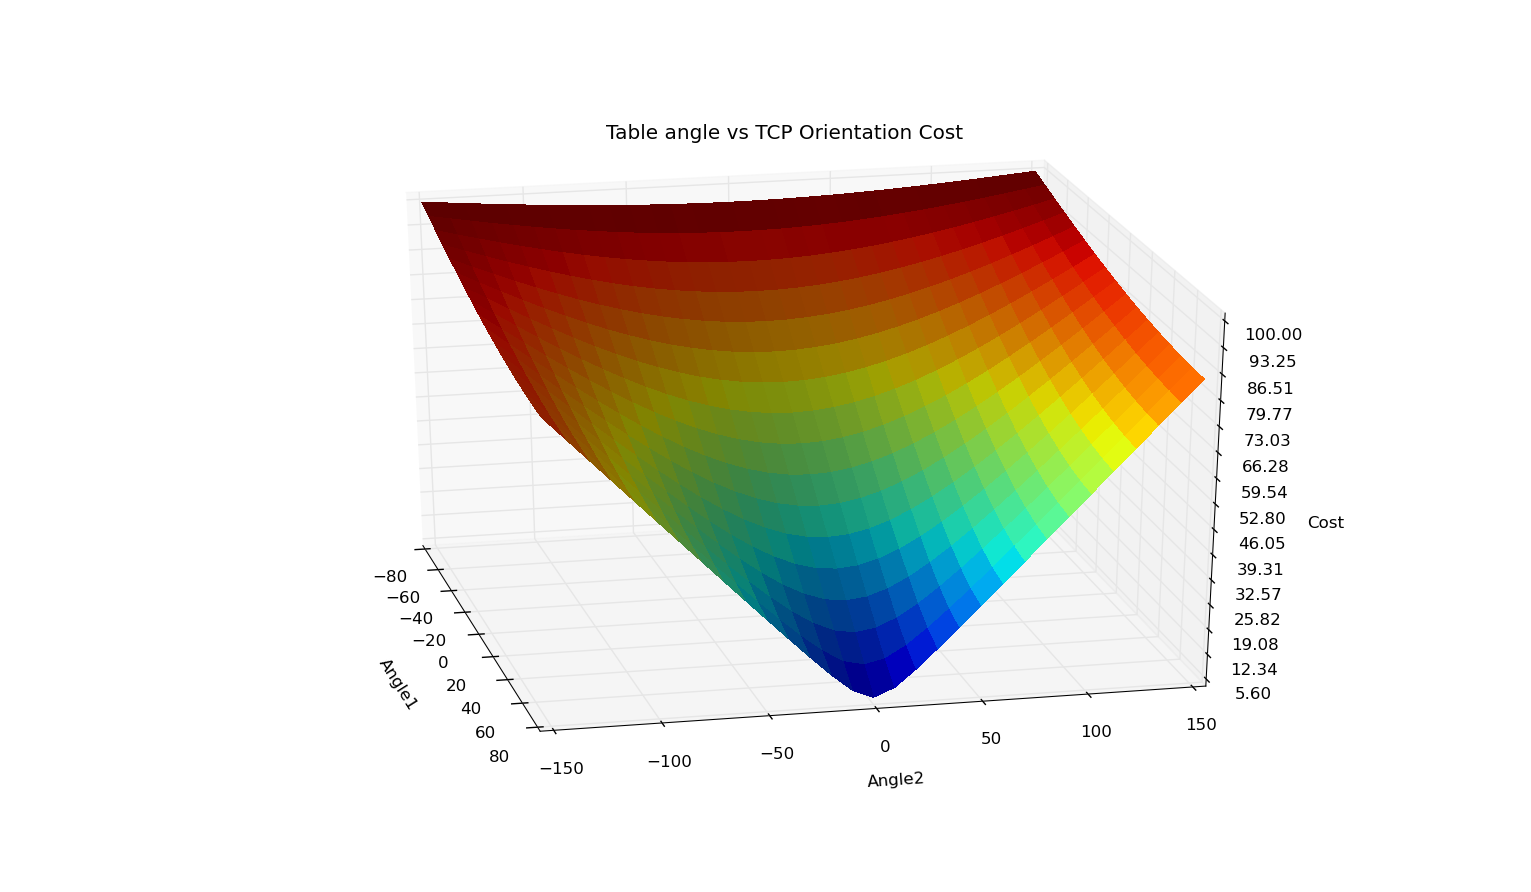
\includegraphics[width=\textwidth]{images/cost_plot3.png}}
   \caption{Cost Plot of Table Angle vs TCP Orientation}
\label{fig:img14}
\end{figure}
\paragraph{2nd Work Piece}
\subparagraph{1st Edge}

\begin{figure}[!htbp] %  figure placement: here, top, bottom, or page
 \centering
   \frame{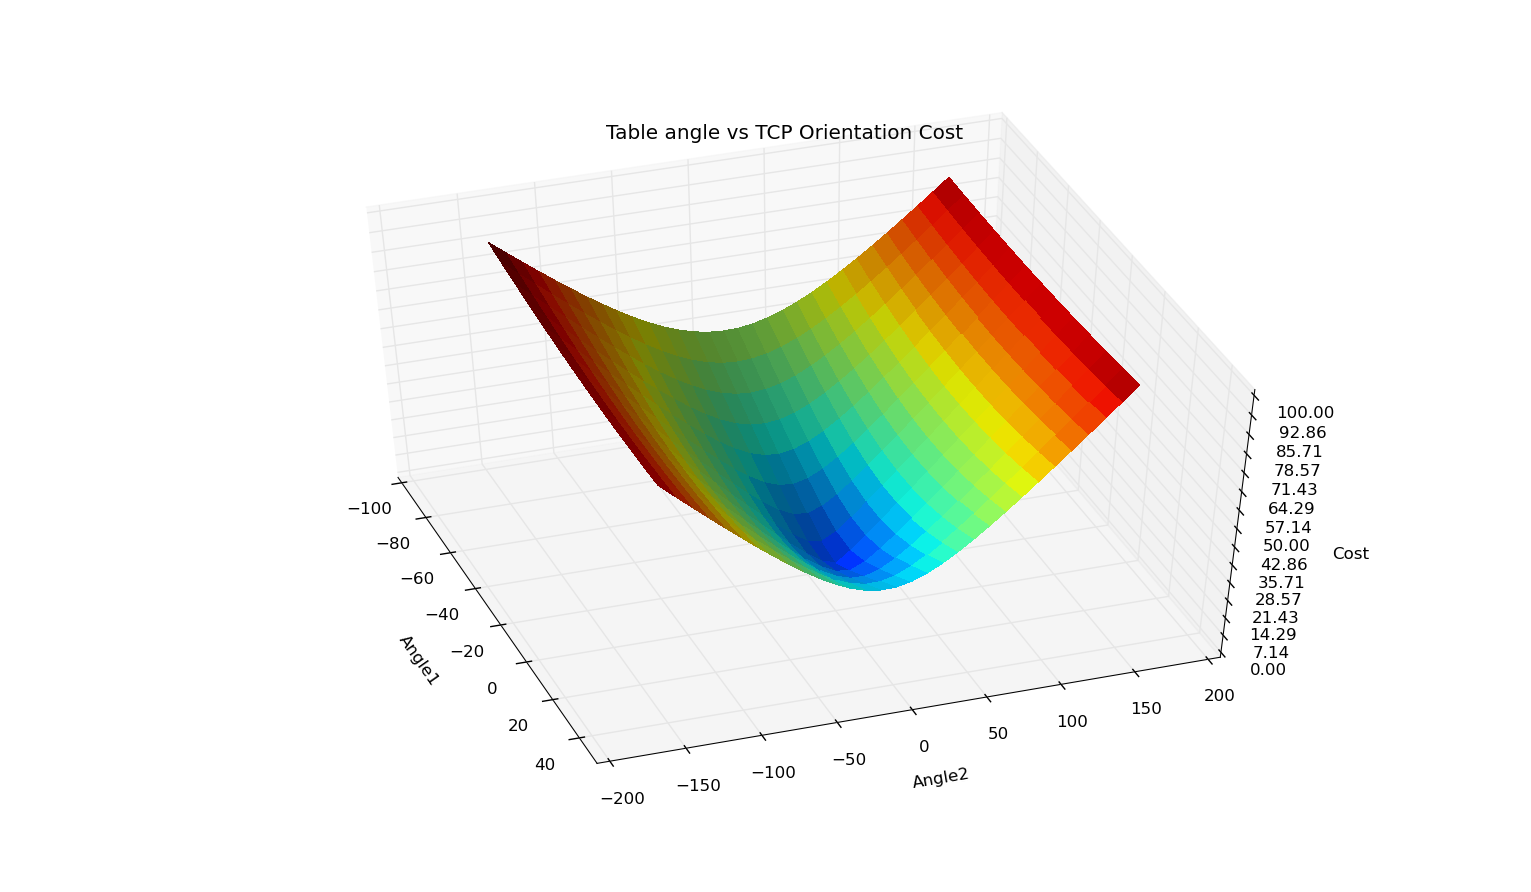
\includegraphics[width=\textwidth]{images/cost_plot5.png}}
   \caption{Cost Plot of Table Angle vs TCP Orientation}  
\label{fig:img15}
\end{figure}
The edge to be welded is marked in yellow(cite fig). In this cost plot(ref img), the minimum cost is obtained when the joints of the table are both at 0$\deg$. In the plot, red represents a higher cost region while blue represents lower cost.
\subparagraph{2nd Edge}
\begin{figure}[!htbp] %  figure placement: here, top, bottom, or page
 \centering
   \frame{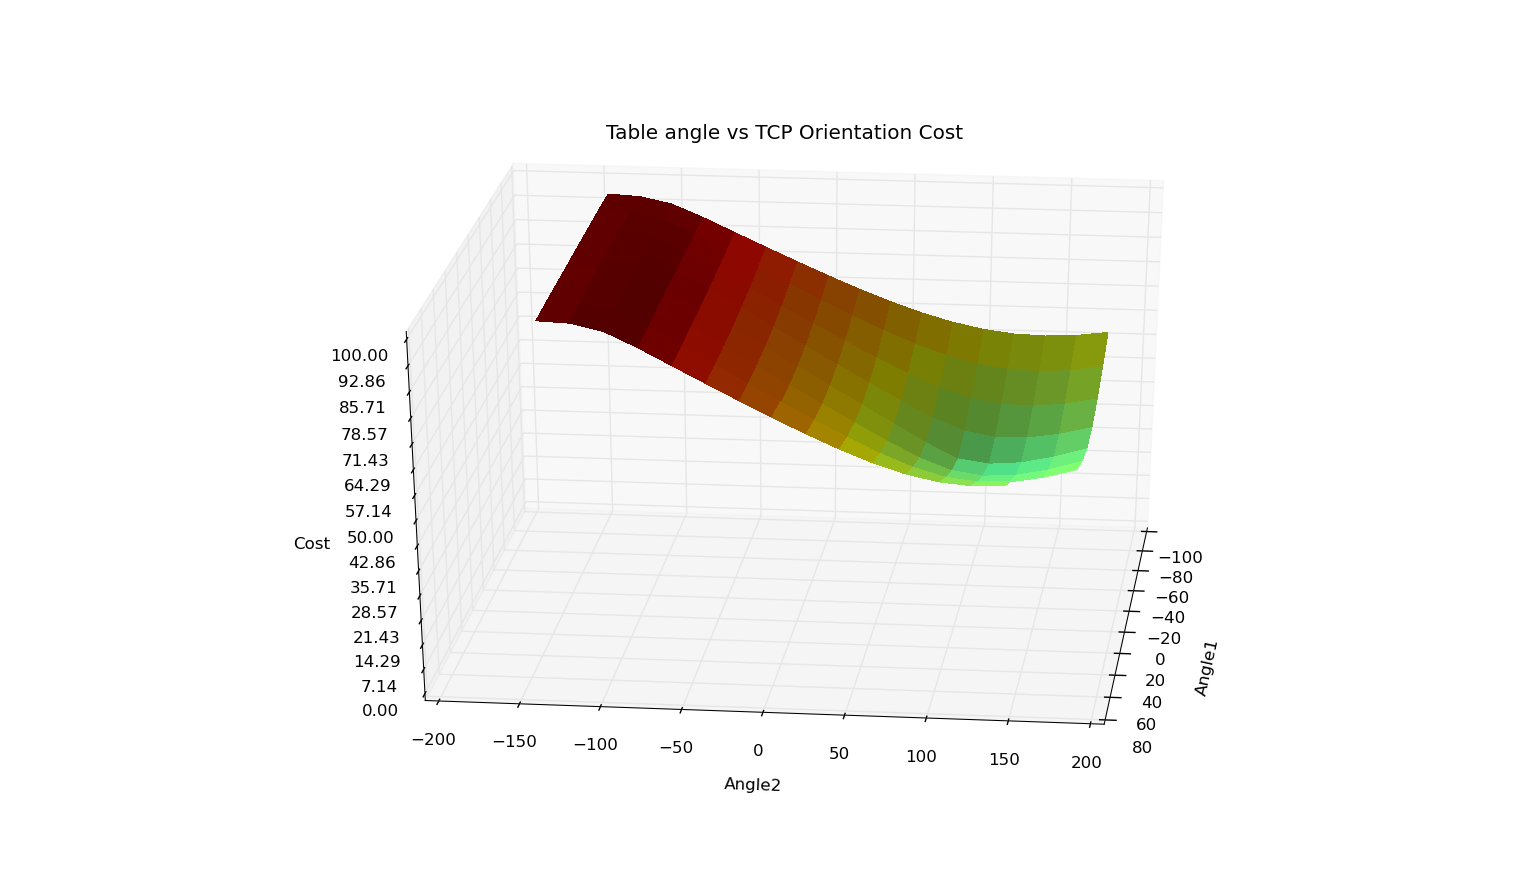
\includegraphics[width=\textwidth]{images/cost_plot7.png}}
   \caption{Cost Plot of Table Angle vs TCP Orientation}
\label{fig:img16}
\end{figure}

\subsubsection{Cost Function based on Joint Movement}
An important criteria of optimizing industrial processes is minimizing the joint movements of a manipulator(cite relevant paper). According to the paper, the more the movement of the bigger joints, the less accurate the process becomes as a small error in the first three joints can propagate to the TCP all the while amplifying its effect, resulting in a gross error.(chng) The following cost function, is defined as follows (write equation.)
\paragraph{1st Work Piece}
\subparagraph{1st Edge}

\begin{figure}[!htbp] %  figure placement: here, top, bottom, or page
 \centering
   \frame{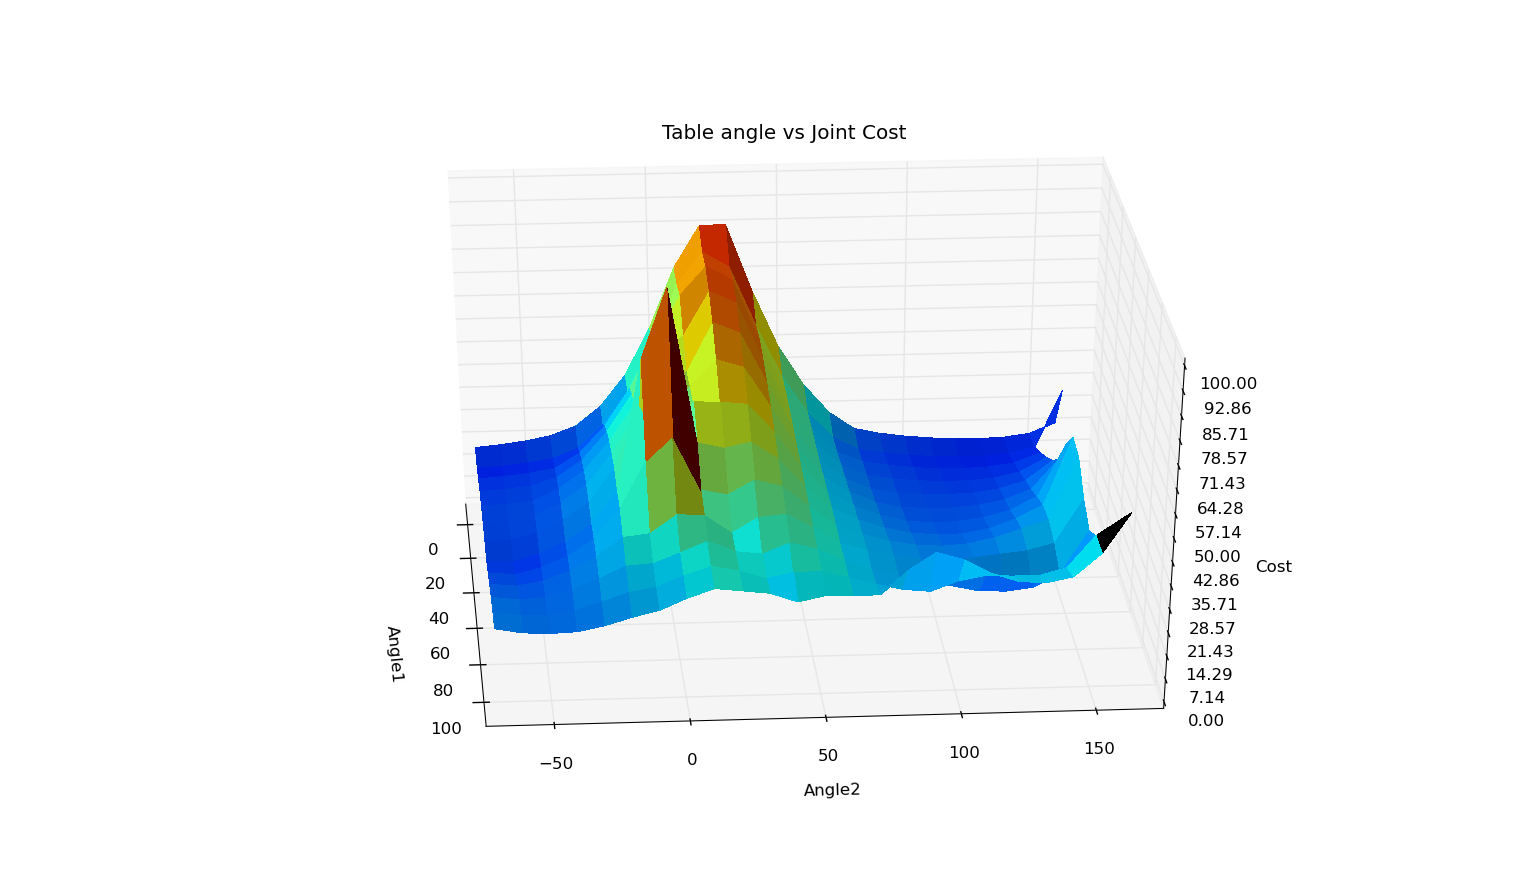
\includegraphics[width=\textwidth]{images/cost_plot2.png}}
   \caption{Cost Plot of Table Angle vs Joint Movement}
\label{fig:img17}
\end{figure}
The edge to be welded is marked in yellow(cite fig). In this cost plot(ref img), the minimum cost is obtained when the joints of the table are both at 0$\deg$. In the plot, red represents a higher cost region while blue represents lower cost.
\subparagraph{2nd Edge}
\begin{figure}[!htbp] %  figure placement: here, top, bottom, or page
 \centering
   \frame{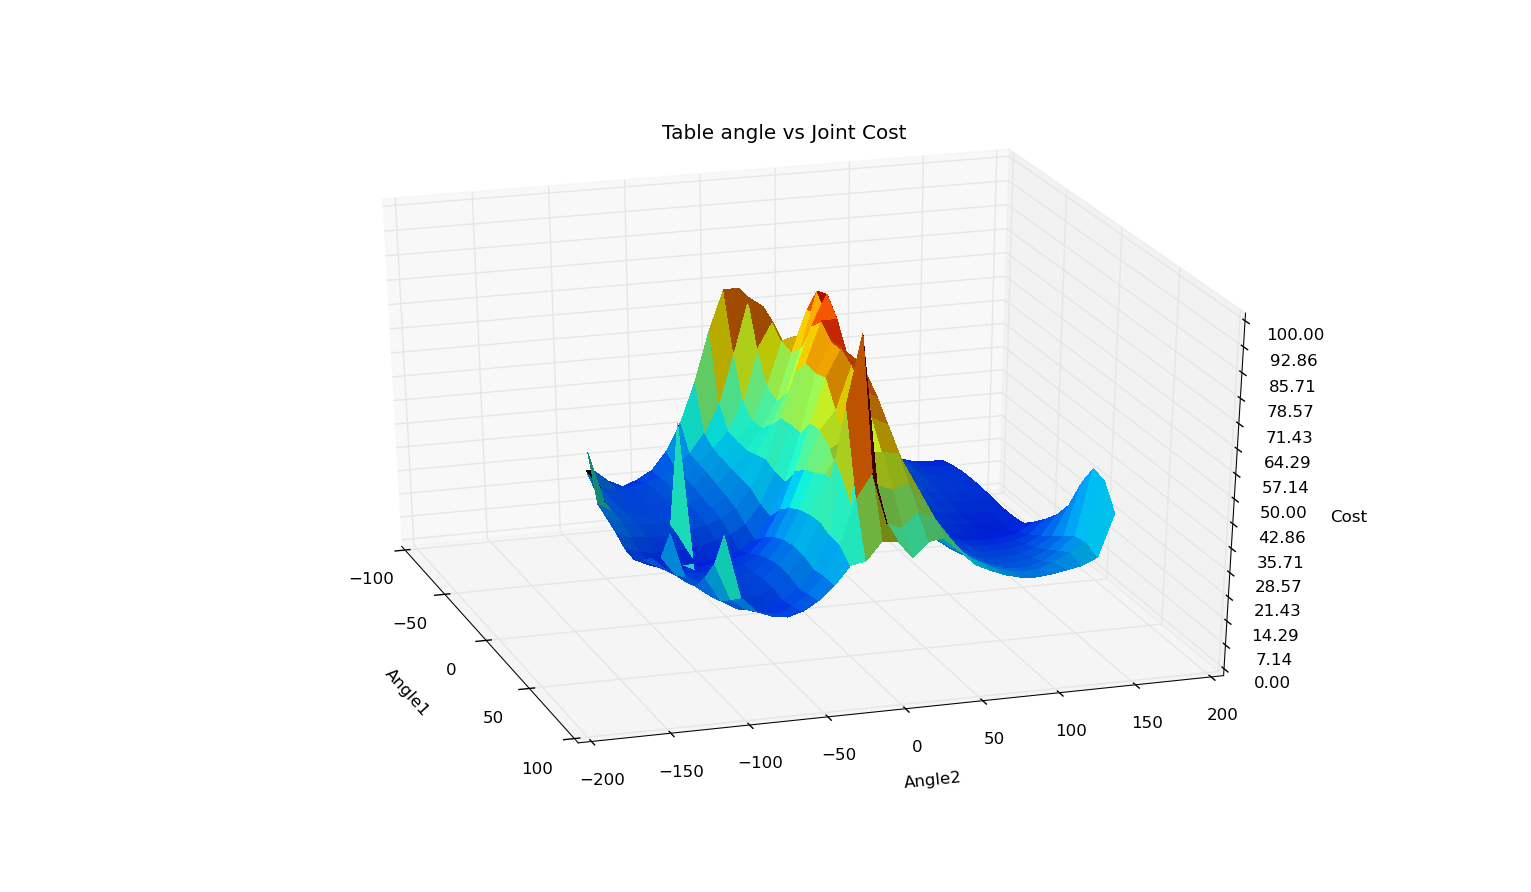
\includegraphics[width=\textwidth]{images/cost_plot4.png}}
   \caption{Cost Plot of Table Angle vs Joint Movement}
\label{fig:img18}
\end{figure}
\paragraph{2nd Work Piece}
\subparagraph{1st Edge}

\begin{figure}[!htbp] %  figure placement: here, top, bottom, or page
 \centering
   \frame{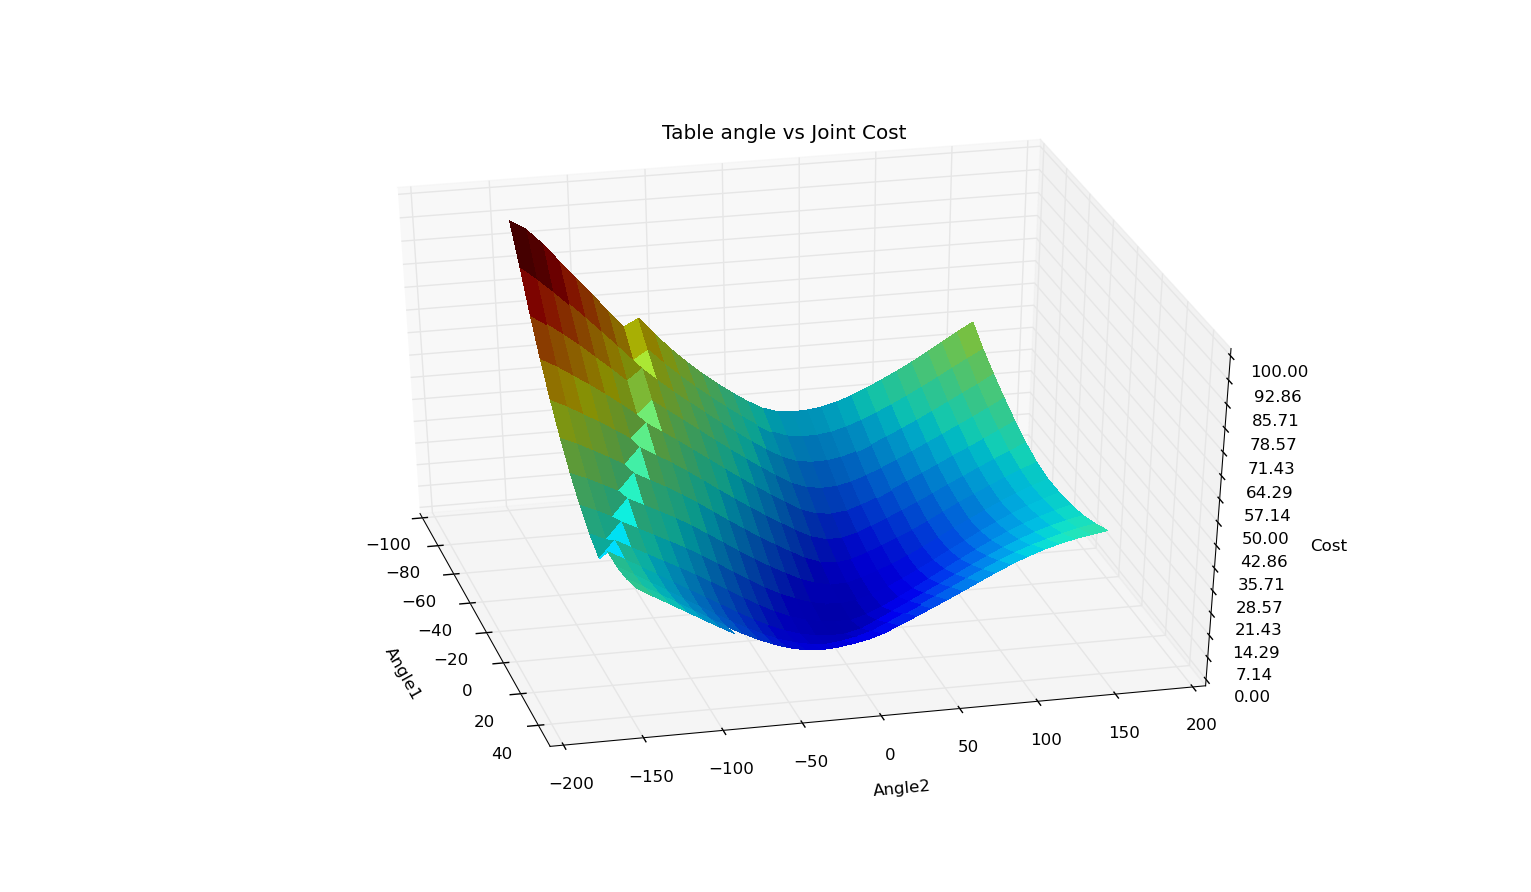
\includegraphics[width=\textwidth]{images/cost_plot6.png}}
   \caption{Cost Plot of Table Angle vs Joint Movement}
\label{fig:img19}
\end{figure}
The edge to be welded is marked in yellow(cite fig). In this cost plot(ref img), the minimum cost is obtained when the joints of the table are both at 0$\deg$. In the plot, red represents a higher cost region while blue represents lower cost.
\subparagraph{2nd Edge}
\begin{figure}[!htbp] %  figure placement: here, top, bottom, or page
 \centering
   \frame{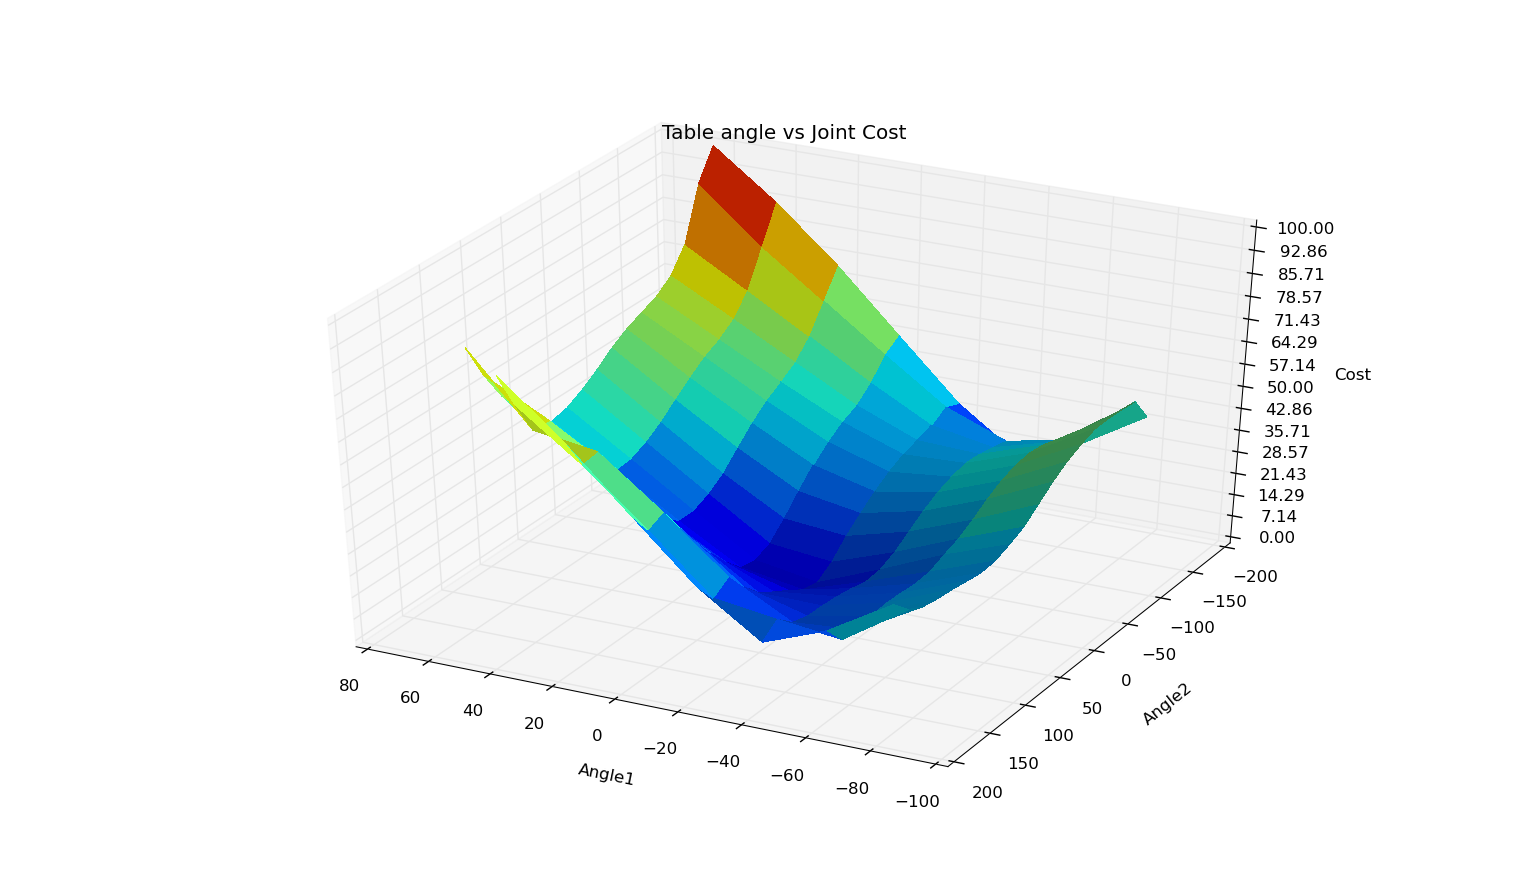
\includegraphics[width=\textwidth]{images/cost_plot8.png}}
   \caption{Cost Plot of Table Angle vs Joint Movement}
\label{fig:img18}
\end{figure}
\subsubsection{Cumulative Cost Function}
\subsection{Optimization Approaches}
\subsubsection{Hill Descent Algorithm Approach}
\subsubsection{Simulated Annealing Algorithm Approach}
\subsection{Comparative Evaluation and Analysis}
